\documentclass[10pt,landscape]{article}
\usepackage{multicol}
\usepackage{calc}
\usepackage{ifthen}
\usepackage[landscape]{geometry}
\usepackage{hyperref}

% To make this come out properly in landscape mode, do one of the following
% 1.
%  pdflatex latexsheet.tex
%
% 2.
%  latex latexsheet.tex
%  dvips -P pdf  -t landscape latexsheet.dvi
%  ps2pdf latexsheet.ps


% If you're reading this, be prepared for confusion.  Making this was
% a learning experience for me, and it shows.  Much of the placement
% was hacked in; if you make it better, let me know...


% 2008-04
% Changed page margin code to use the geometry package. Also added code for
% conditional page margins, depending on paper size. Thanks to Uwe Ziegenhagen
% for the suggestions.

% 2006-08
% Made changes based on suggestions from Gene Cooperman. <gene at ccs.neu.edu>


% To Do:
% \listoffigures \listoftables
% \setcounter{secnumdepth}{0}


% This sets page margins to .5 inch if using letter paper, and to 1cm
% if using A4 paper. (This probably isn't strictly necessary.)
% If using another size paper, use default 1cm margins.
\ifthenelse{\lengthtest { \paperwidth = 11in}}
	{ \geometry{top=.5in,left=.5in,right=.5in,bottom=.5in} }
	{\ifthenelse{ \lengthtest{ \paperwidth = 297mm}}
		{\geometry{top=1cm,left=1cm,right=1cm,bottom=1cm} }
		{\geometry{top=1cm,left=1cm,right=1cm,bottom=1cm} }
	}

% Turn off header and footer
\pagestyle{empty}
 

% Redefine section commands to use less space
\makeatletter
\renewcommand{\section}{\@startsection{section}{1}{0mm}%
                                {-1ex plus -.5ex minus -.2ex}%
                                {0.5ex plus .2ex}%x
                                {\normalfont\large\bfseries}}
\renewcommand{\subsection}{\@startsection{subsection}{2}{0mm}%
                                {-1explus -.5ex minus -.2ex}%
                                {0.5ex plus .2ex}%
                                {\normalfont\normalsize\bfseries}}
\renewcommand{\subsubsection}{\@startsection{subsubsection}{3}{0mm}%
                                {-1ex plus -.5ex minus -.2ex}%
                                {1ex plus .2ex}%
                                {\normalfont\small\bfseries}}
\makeatother

% Define BibTeX command
\def\BibTeX{{\rm B\kern-.05em{\sc i\kern-.025em b}\kern-.08em
    T\kern-.1667em\lower.7ex\hbox{E}\kern-.125emX}}

% Don't print section numbers
\setcounter{secnumdepth}{0}


\setlength{\parindent}{0pt}
\setlength{\parskip}{0pt plus 0.5ex}


% -----------------------------------------------------------------------

\title{ELEC 460 CheatSheet}
\usepackage{lmodern}           % fonts
\usepackage{amssymb,amsmath}   % math equations
%\usepackage{parskip}           % no paragraph skip
\usepackage[american,siunitx]{circuitikz}        % Circuits, drawing
\usepackage{booktabs}          % Fancy tables
%\usepackage{float}             % float for figure and tables

\usepackage{rotating}
\usepackage{tikz}
\begin{document}
\begin{multicols}{2}

\subsection{Z-transform}
\begin{tabular}{p{7.75cm} p{4.75cm}}
$\mathcal{Z} \left\{ f_1(t) \pm f_2(t) \right\}=F_1(z)+F_2(z)$ & Addition\\
$\mathcal{Z} \left\{ af(t) \right\}= aF(z)$ & Multiplication by a Constant \\
$\mathcal{Z} \left\{ f(t-nT) \right\}=z^{-n}F(z)$ & Shifting \\
$\mathcal{Z} \left\{ f(t+kT) \right\}=z^{k}F(z)-z^{k}f(0)- \cdots - z f(kT-T)$ & Shifting (cont'd)\\
$\mathcal{Z} \left\{ e^{\mp at} f(t) \right\}=F(ze^{\pm at})$ & Complex Translation \\
$\lim_{k \rightarrow \infty} f(kT)= \lim_{z \rightarrow 0}F(z)$ & Initial Value Theorem \\ \hline
If $(1-z^{-1})F(z)$ has all singularities inside unit disk $|z|=1$, then & Final Value Theorem \\
$\lim_{k \rightarrow \infty} f(kT) = \lim_{z \rightarrow 1} (1-z^{-1})F(z)$ & \\
$\mathcal{Z} \left\{ \frac{\partial}{\partial a} f(t,a) \right\} = \frac{\partial}{\partial a} F(z,a)$& Partial differentiation
\end{tabular}

\subsection{Sampling Theory}
\vspace*{-0.25cm}
\begin{align*}
& \mathcal{Z} \left\{G_1(s)G_2(s)\right\}=G_1G_2(z)= G_2G_1(z) \quad \text{In General} \quad G_1(z)G_2(z) \neq G_1G_2(z)
\end{align*}
\vspace*{-0.175cm}
\begin{minipage}[t]{1\linewidth}
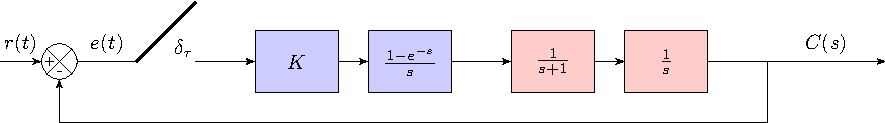
\includegraphics[width=1\linewidth]{samplerTesting-cropped.pdf}
\end{minipage}
\begin{align*}
& G(z) = \mathcal{Z} \left\{\left(\frac{1-e^{-s}}{s}\right) \left[ \frac{1}{s+1}\right] \left[\frac{1}{s}\right] \right\} \rightarrow G_1(z) = (1-z^{-1})\mathcal{Z} \left\{ G_{rest}(s) \right\}
\end{align*}
\begin{minipage}[h]{0.65\linewidth}
%\medbreak\noindent\minipage{\columnwidth}
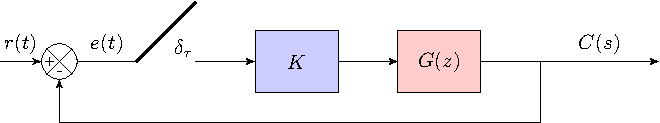
\includegraphics[width=1.05\linewidth]{sampleEND-cropped.pdf}%\endminipage\medbreak
\end{minipage}
\begin{minipage}[h]{0.35\linewidth}
\[
G(z) = \frac{ze^{-1}+(1-ze^{-1})}{(z-1)(z-e^{-1})} 
\]
\end{minipage}
$$ \text{ZOH(zero-hold-system)} \quad 
f^\ast(t) = \sum_{k=-\infty}^\infty f(kT)\delta(t-kT)  \quad 
G_{h}(s)= \frac{1-e^{-Ts}}{s}
$$
\subsection{Stability Test for Digital Systems}
\vspace*{-0.45cm}
\begin{align*}
& P(z) = a_0z^n+a_1z^{n-1} + \cdots + a_{n-1}z+a_n \quad G(z)= \frac{A(z)}{P(z)} \\
& \text{Stability Condition:} \quad P(z) \neq 0 \quad |z| \geq 1 \quad (\text{Draw Unit Circle to test stability})\\
& \text{Routh-Stability in Digital Domain: } s = \frac{z+1}{z-1} \quad z=\frac{s+1}{s-1}
\end{align*}
%\begin{table}
%\captionof{Table}{Jury-Marden Table}
\textbf{Jury-Marden Table Uses function P of z} \newline
%\vspace*{-0.25cm}
\begin{minipage}[t]{1\linewidth}
\begin{minipage}[h]{0.25\linewidth}
\begin{align*}
& b_k = \det \begin{bmatrix}
a_n & a_{n-1-k} \\
a_0 & a_{k+1}
\end{bmatrix} \\
& k = 0,1,  \cdots n-1 \\
& c_k = \det \begin{bmatrix}
b_{n-1} & b_{n-2-k} \\
b_0 & b_{k+1}
\end{bmatrix} \\
& k = 0,1,  \cdots n-1 \\
& q_k = \det \begin{bmatrix}
p_{3} & p_{2-k} \\
p_0 & p_{k+1}
\end{bmatrix} \\
& k =0,1,2
\end{align*}
\end{minipage}
\begin{minipage}[h]{0.75\linewidth}
\begin{tabular}{llllllll}
%\cline{1-5}
Row & $z^0$     & $z^1$     & $z^2$     &          & $z^{n-2}$ & $z^{n-1}$ & $z^n$ \\ %\cline{1-5}
1   & $a_n$     & $a_{n-1}$ & $a_{n-2}$ & $\cdots$ & $a_2$     & $a_1$     & $a_0$ \\
2   & $a_0$     & $a_1$     & $a_2$     & $\cdots$ & $a_{n-2}$ & $a_{n-1}$ & $a_n$ \\
3   & $b_{n-1}$ & $b_{n-2}$ & $b_{n-3}$ & $\cdots$ & $b_1$     & $b_0$     &       \\ %\cline{1-5}
4   & $b_0$     & $b_1$     & $b_2$     & $\cdots$ & $b_{n-2}$ & $b_{n-1}$ &       \\
5   & $c_{n-2}$ & $c_{n-3}$ & $c_{n-4}$ & $\cdots$ & $c_0$     &           &       \\
6   & $c_0$     & $c_1$     & $c_2$     & $\cdots$ & $c_{n-2}$ &           &      \\
2n-5& $p_3$ & $p_2$ & $p_1$ & $p_0$ & & \\
2n-4& $p_0$ & $p_1$ & $p_2$ & $p_3$ & & \\
2n-3& $q_2$ & $q_1$ & $q_0$ & & & 
\end{tabular}
\end{minipage}
\end{minipage}

\textbf{Necessary and Sufficient Condition for Stability} \newline
\begin{minipage}[h]{0.55\linewidth}
\begin{enumerate}
\item $|a_n| < |a_0|$ 
\item $P(1) > 0$
\item \begin{align*}
P(-1) & > 0 \ \text{for n even } \\
& < 0 \ \text{for n odd}
\end{align*}
\item $b_{n-1}> |b_0|, |c_{n-2}|>|c_0|, \cdots |q_2| > |q_0|$
\end{enumerate}
\end{minipage}
\begin{minipage}[h]{0.5\linewidth}
\textbf{Special Case n =2} \newline 
$P(z) =a_0z^2+a_1z+a_2$ \newline 
\begin{tabular}{c c c}
$z^0$ & $z^1$& $z^2$ \\
$a_2$ & $a_1$ & $a_0$
\end{tabular} \newline
$P(z) \neq 0$ for $|z| \geq 1$ if and only if 
\begin{enumerate}
\item $|a_2| < |a_0|$
\item $P(1) > 0$
\item $P(-1) > 0 \quad (n=2)$
\end{enumerate}
\end{minipage}

\textbf{Root Locus} presents the poles of the closed loop system when the gain K changes from zero to infinity.

\textbf{Construction of the Root Locus}

Open loop transfer function
$ \displaystyle \text{KH}\left( s \right)G\left( s \right) = K\frac{B(s)}{A(s)}$

m: the order of the \textbf{open-loop} numerator polynomial.

n: the order of the \textbf{open-loop} denominator polynomial. $q=n-m$

\textbf{Rule 1:} number of branches equals the number of poles of the
 open-loop transfer function

\textbf{Rule 2:} If the total number of poles and zeros of the open-loop
 system to the right of the s-point on the real axis is odd, then this
 point lies on the locus.

\textbf{Rule 3:} The locus starting point (K=0) are at the open-loop
poles and the locus ending points (K=$\infty$) are at the open loop zeros and
n-m branches terminate at infinity.

\textbf{Rule 4 and 5:} Slope of asymptotes of root locus as `s' approaches infinity. \newline Abscissa of the intersection between asymptotes of root locus and real-axis.
\[\sigma  = {\frac{\sum\limits_{i = 1}^n {{p_i}}  - \sum\limits_{i = 1}^m {{z_i}} }{q}} \quad \theta = \pm r{\frac{180}{q}} \quad \text{where r=1, 3, 5} \]

%\textbf{Rule 5:} 

\textbf{Rule 6:} Break-away and break-in points. From the characteristic
equation

\[f\left( s \right) = A\left( s \right) + KB\left( s \right) = 0\ \ \ \ and\ \ \ \ K = - \frac{A\left( s \right)}{B\left( s \right)}\]

The break-away and break-in points can be found from

\[\frac{\text{dK}}{\text{ds}} = - \frac{A^{'}\left( s \right)B\left( s \right) - A\left( s \right)B^{'}\left( s \right)}{B^{2}\left( s \right)} = 0
\]

\textbf{Rule 7:} Angle of departure from complex poles or zeros.
Subtract from $180^o$ the sum of all angles from all other zeros and poles
of the open-loop system to the complex pole (or zero) with appropriate signs. 

\[ \text{Z-transform: Definition} \quad F(z)=Z[f(t)]-Z[f(kT)]=\sum_{k=0}^{\infty}f(kT)z^{-k}\]
\end{multicols}
\newpage
\begin{multicols}{3}
\begin{align*}
& e^\ast(\infty)=\lim_{z \rightarrow 1} (1-z^{-1})E(z) \\
& K_p=\lim_{z \rightarrow 1} G(z), \quad e^\ast (\infty) = \frac{1}{1+K_p} \\
& e^\ast(\infty) = \frac{1}{K_v}, \quad K_v = \frac{1}{T} \lim_{z \rightarrow 1}(z-1) G(z)  \\
& e^\ast(\infty) = \frac{1}{K_a}, \quad K_a = \frac{1}{T^2} \lim_{z \rightarrow 1}(z-1)^2 G(z)
\end{align*}

{\bf Linear Factor Rule.}  
For each factor of $Q$ of the form $(ax+b)^m$, 
the partial fraction decomposition contains 
the following sum of $m$ partial fractions:  
\[
\frac{A_1}{ax+b} + \frac{A_2}{(ax+b)^2} + \cdots + \frac{A_m}{(ax+b)^m},
\]
where the $A_i$ are constants to be determined.  

\medskip
\noindent
{\bf Quadratic Factor Rule.}  
For each factor of $Q$ of the form $(ax^2+bx+c)^m$, 
where $ax^2+bx+c$ is an irreducible quadratic, 
the partial fraction decomposition contains 
the following sum of $m$ partial fractions:  
\[
\frac{A_1x+B_1}{ax^2+bx+c} + \frac{A_2x+B_2}{(ax^2+bx+c)^2} + \cdots 
  + \frac{A_mx+B_m}{(ax^2+bx+c)^m},
\]
where the $A_i$ and $B_i$ are constants to be determined. 
\begin{align*}
& x(k+2)-\frac{3}{2}x(k+1)+\frac{1}{2}x(k)=u(k), \text(x(0)=1,x(1)=5/2) \\
& [z^2X(z)-z^2x(0)-zx(1)]-\frac{3}{2}(zX(z)-zx(0)]+\frac{1}{2}X(z)=\frac{z}{z-1} \\
& [z^2-1.5z+0.5z]X(z)= \frac{z}{z-1}+z^2+(2.5-1.5)z \\
& X(z) = \frac{z[1+(z+1)(z-1]}{(z-1)(z-1)(z-0.5)}=\frac{z^3}{(z-1)^2(z-0.5)} \\
& \frac{X(z)}{z}=\frac{z^2}{(z-1)^2(z-0.5)}=\frac{A_{11}}{(z-1)^2}+\frac{A_{12}}{z-1}+\frac{A_{13}}{z-0.5}
\end{align*}
Geometric Sum $\sum\limits_{k = -N}^{N} {ar^{k - 1} = a\frac{1-r^{N}}{{1 - r}}} \sum_{i=0}^\infty a^i=\frac{1}{1-a}$
\textbf{Example Partial Fractions}
\begin{align*}
& \frac{20}{\left(s+3\right)\,\left(s^2+6\,s+25\right)} \rightarrow 
\frac{5}{4\,\left(s+3\right)}-\frac{\frac{5\,s}{4}+\frac{15}{4}}{s^2+6\,s+25} \\
& \frac{5\,z}{4\,\left(z-{\mathrm{e}}^{-3}\right)}+\frac{5\,z\,{\mathrm{e}}^3\,\left(\cos\left(4\right)-z\,{\mathrm{e}}^3\right)}{4\,\left({\mathrm{e}}^6\,z^2-2\,\cos\left(4\right)\,{\mathrm{e}}^3\,z+1\right)} \ \text{Z-table} = \text{17}
\end{align*}
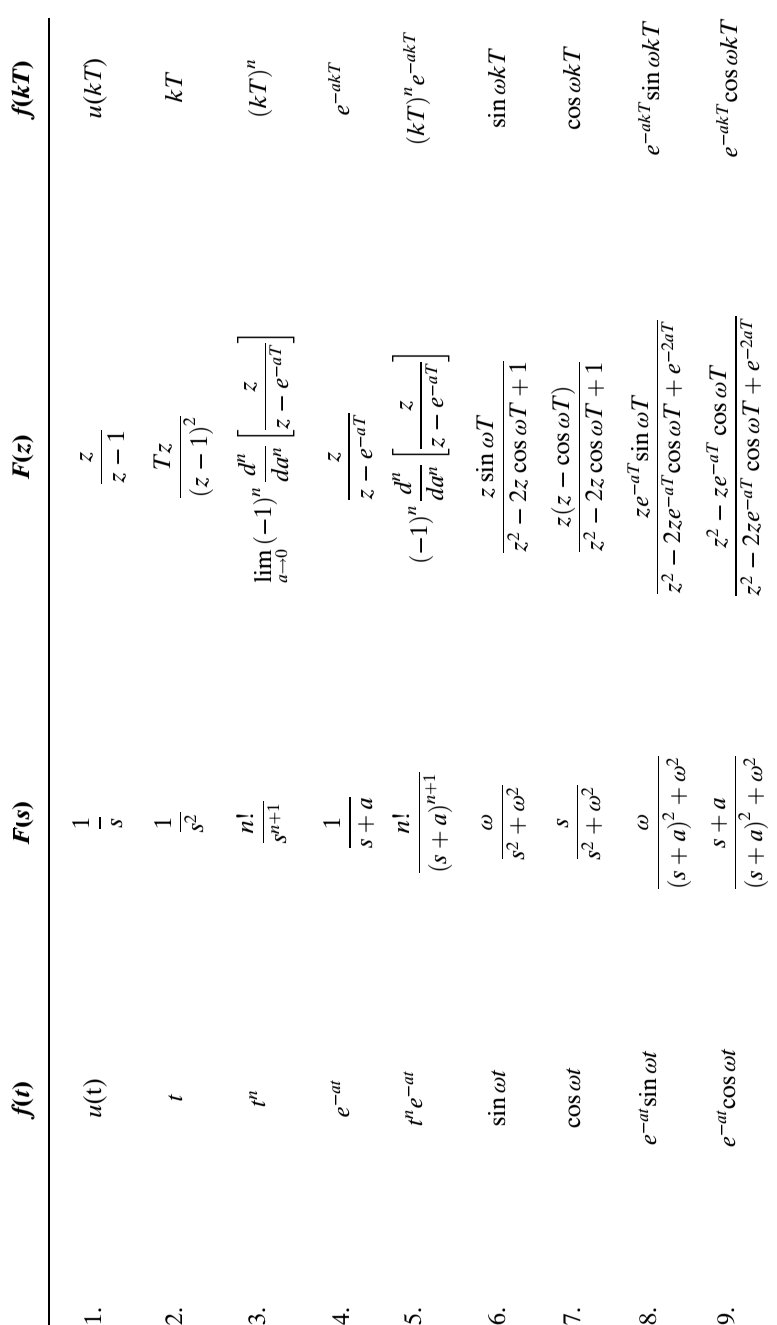
\includegraphics[width=1\linewidth]{NICEPictureRotate.png}
$\text{Ch.eqn} =\Delta P(z)=z^2+(K-4)z+0.8=0$ \newline
Inputting $z=1 \text{ and } z=-1$, $K=-0.8-1+4=2.2$, $K=(1)^2+4+0.8=5.8$, for stability $-1<K<1$.
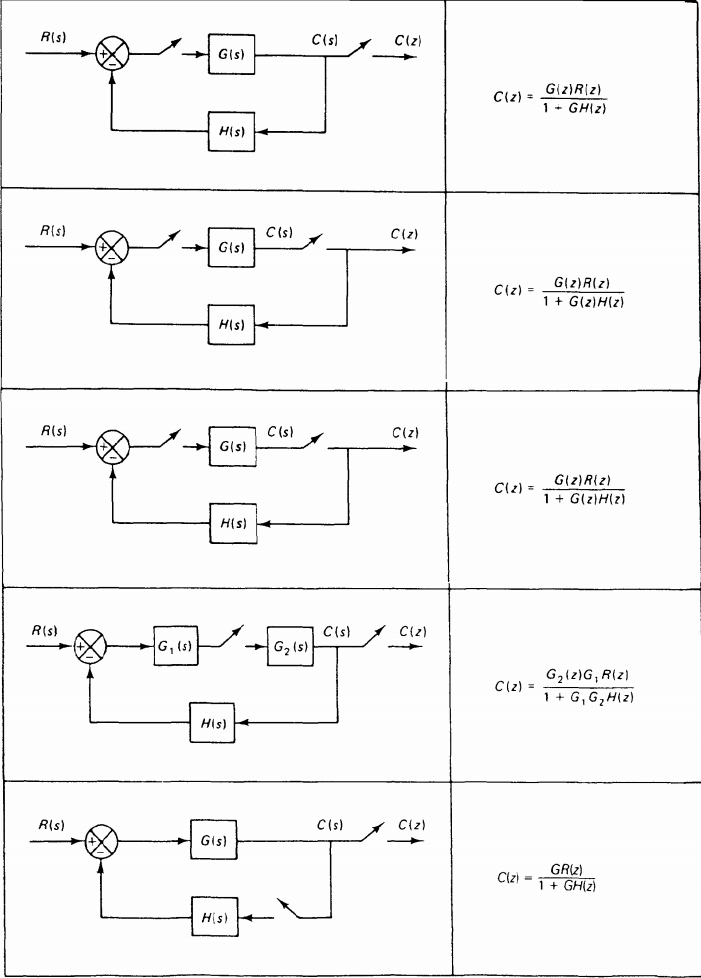
\includegraphics[width=1\linewidth]{OgataTable.png}
% \begin{align*}
% & G_p(s)=\frac{K}{s(s+3)} \rightarrow \frac{1}{s(s+3)}
% \end{align*}
%https://www.wolframalpha.com/input/?i=Plot++(t-2)*heaviside(t-2)-+(t-5)*heaviside(t-5)
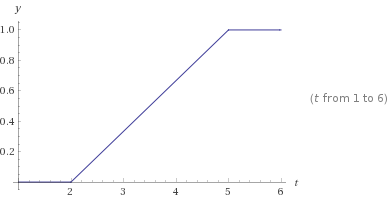
\includegraphics[width=1\linewidth]{heavsidePlot.png}
\begin{align*}
& \frac{1}{3}((t-2)u(t-2)- (t-5)u(t-5)) \rightarrow \frac{z^2 + z + 1}{3 (z - 1) z^4} \\
& =
\frac{1(z^{-3}+z^{-4}+z^{-5})}{3(1-z^{-1})} \quad \frac{1}{3}z^{-3}+\frac{2}{3}z^{-4}+z^{-5}+z^{-6}+ \cdots 
\end{align*}
\end{multicols}

\newpage
\begin{sidewaysfigure}
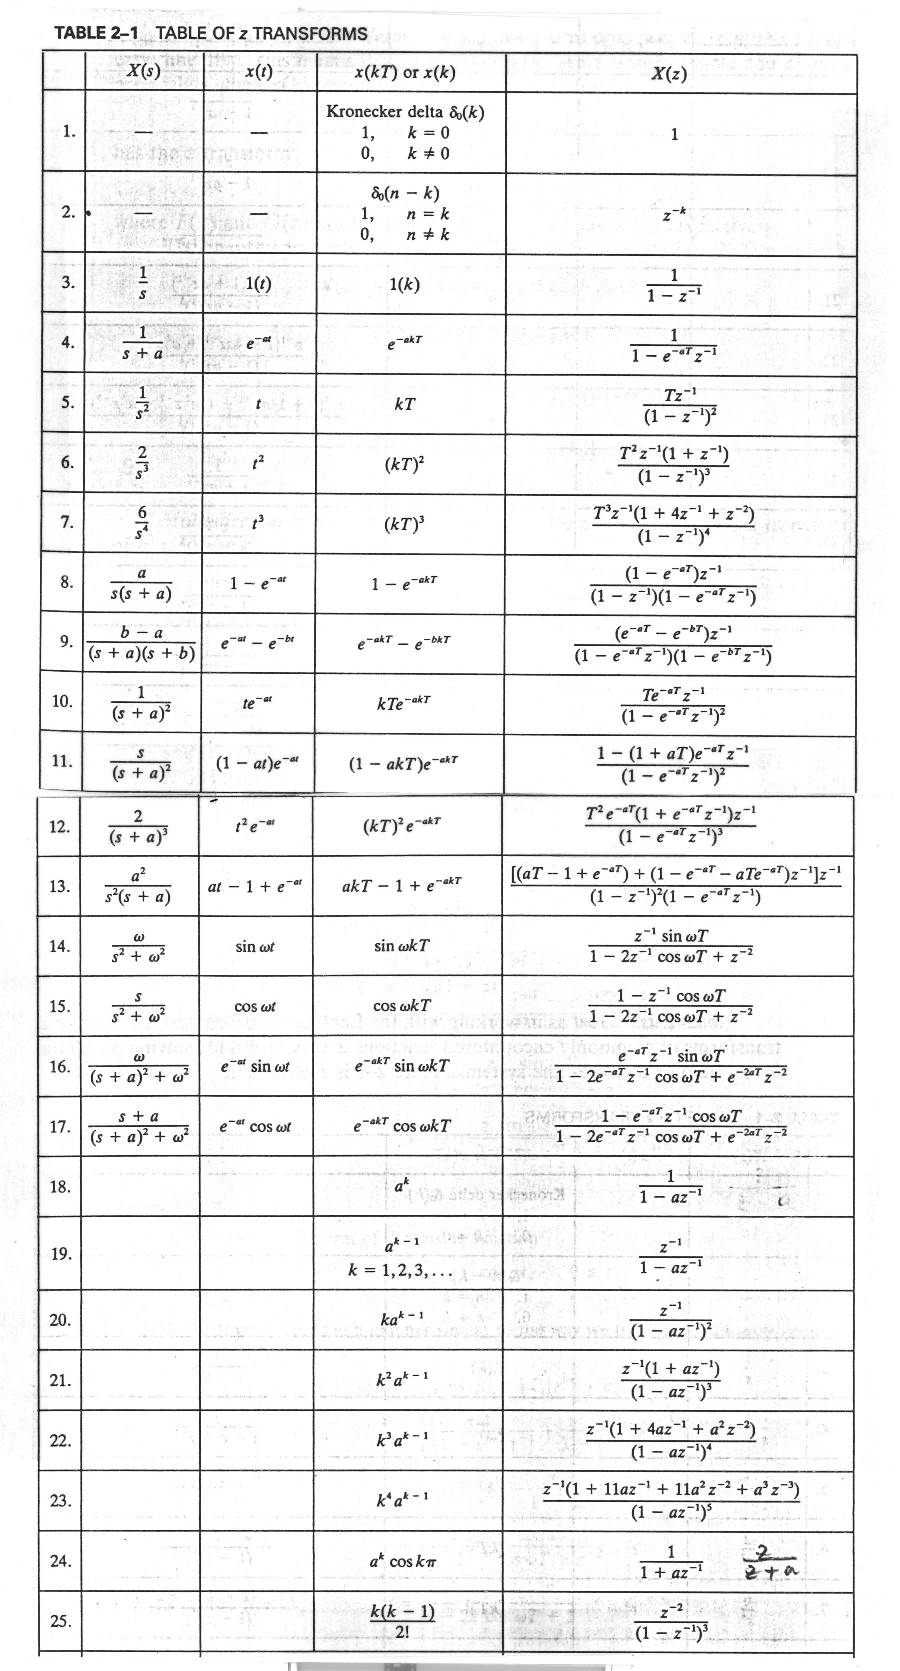
\includegraphics[width=0.75\linewidth]{Table_z_Transforms.pdf}
\end{sidewaysfigure}
%\end{table}

    
\end{document}